
\documentclass[a4paper,11pt]{article}
\usepackage[a4paper, margin=8em]{geometry}

% usa i pacchetti per la scrittura in italiano
\usepackage[french,italian]{babel}
\usepackage[T1]{fontenc}
\usepackage[utf8]{inputenc}
\frenchspacing 

% usa i pacchetti per la formattazione matematica
\usepackage{amsmath, amssymb, amsthm, amsfonts}

% usa altri pacchetti
\usepackage{gensymb}
\usepackage{hyperref}
\usepackage{standalone}

% imposta il titolo
\title{Appunti Elettronica Digitale}
\author{Luca Seggiani}
\date{2026}

% imposta lo stile
% usa helvetica
\usepackage[scaled]{helvet}
% usa palatino
\usepackage{palatino}
% usa un font monospazio guardabile
\usepackage{lmodern}

\renewcommand{\rmdefault}{ppl}
\renewcommand{\sfdefault}{phv}
\renewcommand{\ttdefault}{lmtt}

% disponi il titolo
\makeatletter
\renewcommand{\maketitle} {
	\begin{center} 
		\begin{minipage}[t]{.8\textwidth}
			\textsf{\huge\bfseries \@title} 
		\end{minipage}%
		\begin{minipage}[t]{.2\textwidth}
			\raggedleft \vspace{-1.65em}
			\textsf{\small \@author} \vfill
			\textsf{\small \@date}
		\end{minipage}
		\par
	\end{center}

	\thispagestyle{empty}
	\pagestyle{fancy}
}
\makeatother

% disponi teoremi
\usepackage{tcolorbox}
\newtcolorbox[auto counter, number within=section]{theorem}[2][]{%
	colback=blue!10, 
	colframe=blue!40!black, 
	sharp corners=northwest,
	fonttitle=\sffamily\bfseries, 
	title=~\thetcbcounter: #2, 
	#1
}

% disponi definizioni
\newtcolorbox[auto counter, number within=section]{definition}[2][]{%
	colback=red!10,
	colframe=red!40!black,
	sharp corners=northwest,
	fonttitle=\sffamily\bfseries,
	title=~\thetcbcounter: #2,
	#1
}

% U.D.M
\newcommand{\amp}{\ensuremath{\mathrm{A}}}
\newcommand{\volt}{\ensuremath{\mathrm{V}}}
\newcommand{\meter}{\ensuremath{\mathrm{m}}}
\newcommand{\second}{\ensuremath{\mathrm{s}}}
\newcommand{\farad}{\ensuremath{\mathrm{F}}}
\newcommand{\henry}{\ensuremath{\mathrm{H}}}
\newcommand{\siemens}{\ensuremath{\mathrm{S}}}

% circuiti
\usepackage{circuitikz}
\usetikzlibrary{babel}

% disegni
\usepackage{pgfplots}
\pgfplotsset{width=10cm,compat=1.9}

% disponi codice
\usepackage{listings}
\usepackage[table]{xcolor}

\definecolor{codegreen}{rgb}{0,0.6,0}
\definecolor{codegray}{rgb}{0.5,0.5,0.5}
\definecolor{codepurple}{rgb}{0.58,0,0.82}
\definecolor{backcolour}{rgb}{0.95,0.95,0.92}

\lstdefinestyle{codestyle}{
		backgroundcolor=\color{black!5}, 
		commentstyle=\color{codegreen},
		keywordstyle=\bfseries\color{magenta},
		numberstyle=\sffamily\tiny\color{black!60},
		stringstyle=\color{green!50!black},
		basicstyle=\ttfamily\footnotesize,
		breakatwhitespace=false,         
		breaklines=true,                 
		captionpos=b,                    
		keepspaces=true,                 
		numbers=left,                    
		numbersep=5pt,                  
		showspaces=false,                
		showstringspaces=false,
		showtabs=false,                  
		tabsize=2
}

\lstdefinestyle{shellstyle}{
		backgroundcolor=\color{black!5}, 
		basicstyle=\ttfamily\footnotesize\color{black}, 
		commentstyle=\color{black}, 
		keywordstyle=\color{black},
		numberstyle=\color{black!5},
		stringstyle=\color{black}, 
		showspaces=false,
		showstringspaces=false, 
		showtabs=false, 
		tabsize=2, 
		numbers=none, 
		breaklines=true
}

\lstdefinelanguage{javascript}{
	keywords={typeof, new, true, false, catch, function, return, null, catch, switch, var, if, in, while, do, else, case, break},
	keywordstyle=\color{blue}\bfseries,
	ndkeywords={class, export, boolean, throw, implements, import, this},
	ndkeywordstyle=\color{darkgray}\bfseries,
	identifierstyle=\color{black},
	sensitive=false,
	comment=[l]{//},
	morecomment=[s]{/*}{*/},
	commentstyle=\color{purple}\ttfamily,
	stringstyle=\color{red}\ttfamily,
	morestring=[b]',
	morestring=[b]"
}

% disponi sezioni
\usepackage{titlesec}

\titleformat{\section}
	{\sffamily\Large\bfseries} 
	{\thesection}{1em}{} 
\titleformat{\subsection}
	{\sffamily\large\bfseries}   
	{\thesubsection}{1em}{} 
\titleformat{\subsubsection}
	{\sffamily\normalsize\bfseries} 
	{\thesubsubsection}{1em}{}

% disponi alberi
\usepackage{forest}

\forestset{
	rectstyle/.style={
		for tree={rectangle,draw,font=\large\sffamily}
	},
	roundstyle/.style={
		for tree={circle,draw,font=\large}
	}
}

% disponi algoritmi
\usepackage{algorithm}
\usepackage{algorithmic}
\makeatletter
\renewcommand{\ALG@name}{Algoritmo}
\makeatother

% disponi numeri di pagina
\usepackage{fancyhdr}
\fancyhf{} 
\fancyfoot[L]{\sffamily{\thepage}}

\makeatletter
\fancyhead[L]{\raisebox{1ex}[0pt][0pt]{\sffamily{\@title \ \@date}}} 
\fancyhead[R]{\raisebox{1ex}[0pt][0pt]{\sffamily{\@author}}}
\makeatother

\begin{document}
% sezione (data)
\section{Lezione del 17-03-26}

% stili pagina
\thispagestyle{empty}
\pagestyle{fancy}

% testo
Nella scorsa lezione abbiamo visto come usare il diodo in alcuni circuiti elementari, fra cui i \textit{rettificatori}. In particolare, finora abbiamo considerato il comportamento dei rettificatori sottoposti ad un carico resistivo secondo due modelli (ideale e caduta costante). Vediamo cosa succede se si sottpono il rettificatore ad un carico, invece, \textit{reattivo}.

\subsubsection{Circuito rettificatore con condensatore}
Vediamo quindi cosa succede se mettiamo a valel del rettificatore un \textit{condensatore}:
\begin{center}
\begin{circuitikz}
	\draw (0,2) to[american voltage source, l=$V_s$] (0, 0);
	\node[ground] at(0,0) {};
	\draw (0,2) to[diode, l=$D$] (4,2) to[capacitor, l=$C$] (4,0);
	\node[ground] at(4,0) {};
	\draw (4,2) -- (5, 2);
	\node[anchor=west] at(5,2) {$V_u$};
\end{circuitikz}
\end{center}

Quello che accadrà in questo caso è che il condensatore, di equazione:
$$
I_C = C \frac{d V_u}{dt} = I_D
$$
ci porterà in una situazione dove:
\begin{center}
	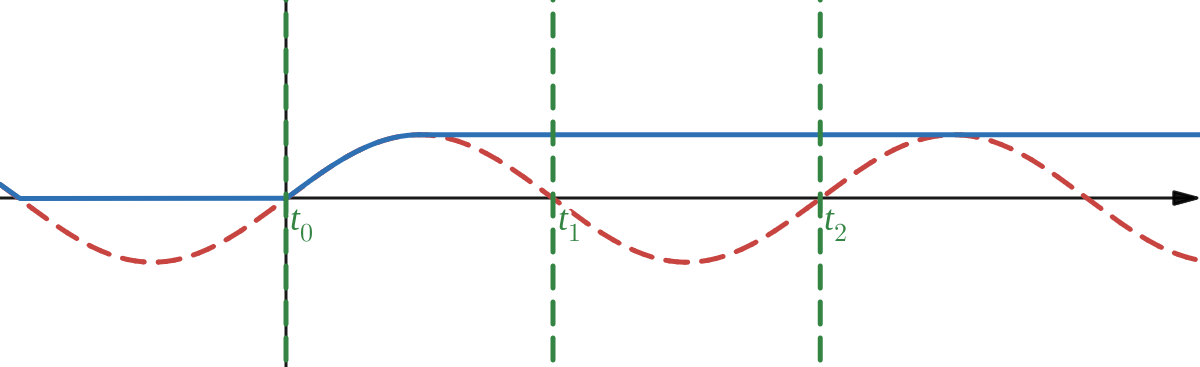
\includegraphics[scale=0.3]{../figures/rect_cap.png}
\end{center}
\begin{enumerate}
	\item Da $t_0$ a $\frac{t_1}{2}$ (considerati gli estremi della scorsa sezione, $\frac{t_1}{2}$ è il picco di tensione) la tensione $V_s$ sarà positiva, e lo sarà anche la $V_u$, che la inseguirà con i vari dettagli che avevamo detto (una piccola caduta di potenziale e il ritardo di conduzoine);
	\item Da $\frac{t_1}{2}$ in poi, se $C$ è abbastanza grande, la capacità vorrà mantenere il voltaggio costante, e quindi avremo che il voltaggio $V_u$ sarà pressappoco costante su $t$. 
\end{enumerate}

In altre parole, ipotizziamo che il diodo si trovi in conduzione finché:
$$
I_D > 0 \implies \frac{d V_u}{dt} > 0
$$
e quindi la $V_u$ caricherà come $V_s$ fino a $\frac{t_1}{2}$. Dopo aver attraversato il primo picco, il condensatore no caricherà più, il diodo si trasformerà in un aperto, e quindi avremo:
$$
I_C = I_D = 0
$$
Cioè da $\frac{t_1}{2}$ in poi il diodo sarà sempre in inversa, meno i punti di cresta dove starà alla soglia di conduzione ma a corrente nulla.

Questo ci sarà utile se il nostro obiettivo era quello di trasformare una tensione alternata in una tensione continua, cioè effettivamente rettificarla ad una sorgente di tensione costante nel tempo. Notiamo però che non abbiamo totalmente risolto il problema, in quanto potrebbero sempre esserci irregolarità nella retta da $\frac{t_1}{2}$ in poi date dalla scarica del condensatore o dal rumore del segnale $V_s$.

\subsubsection{Circuito rettificatore con filtro RC}
Vediamo nel dettaglio cosa intendiamo. Se reintroduciamo una resistenza di carico, in parallelo al condensatore, otteniamo la seguente configurazione:
\begin{center}
\begin{circuitikz}
	\draw (0,2) to[american voltage source, l=$V_s$] (0, 0);
	\node[ground] at(0,0) {};
	\draw (0,2) to[diode, l=$D$] (4,2) to[capacitor, l=$C$] (4,0);
	\draw(4,2) -- (6,2) to[resistor, l=$R_L$] (6,0) -- (4,0);
	\node[ground] at(4,0) {};
	\draw (6,2) -- (7, 2);
	\node[anchor=west] at(7,2) {$V_u$};
\end{circuitikz}
\end{center}

In questo caso il condensatore, da $\frac{t_1}{2}$ in poi, avrà modo di scaricarsi su $R_L$. In altre parole, quando il diodo entrerà in interdizione, la tensione sul condensatore tendera a scaricarsi sulla resistenza seguendo l'equazione tipica del circuito RC:
$$
V_u \propto e^{-\frac{t}{\tau}}, \quad \tau = RC
$$
Ciò significherà che esisterà un istante, precedente al $t_0$ del ciclo successivo, dove $V_s$ salirà sopra il livello raggiunto da $V_u$, ricaricherà il condensatore (alzando il voltaggio nuovamente fino al valore di picco), permettendo che il ciclo continui.
\begin{center}
	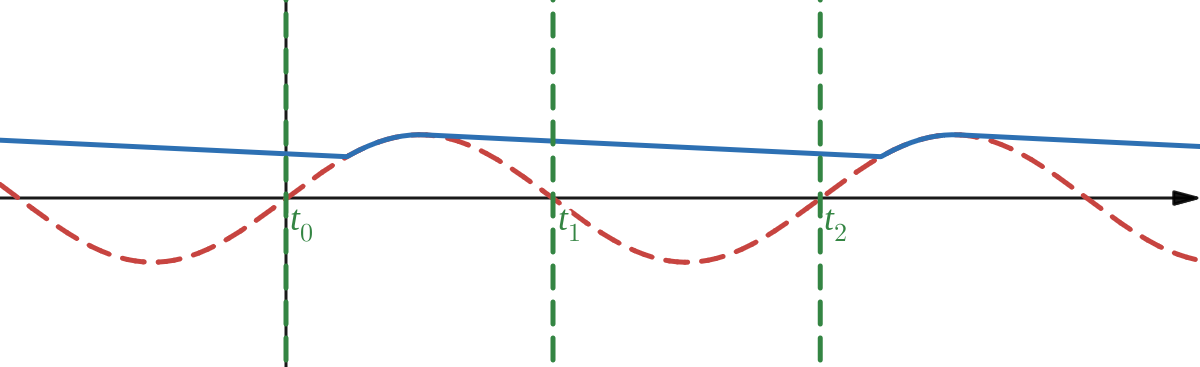
\includegraphics[scale=0.3]{../figures/rect_rc.png}
\end{center}

Chiamiamo questo voltaggio di caduta \textbf{ripple} voltage del rettificatore.

\subsubsection{Circuito rettificatore a doppia semionda}
L'idea che abbiamo guardando al grafico della scorsa sezione è che, se si potessero combinare i contribuiti di due diodi (uno in una direzione, e uno nell'altra, rispetto a $V_s$), allora si potrebe "riempire" il calo di tensione successivo a $\frac{t_1}{2}$ con un contributo in tensione dato dal diodo invertito.

\newpage

Per formalizzare quello che si è detto, introduciamo un componente detto \textbf{trasformatore}, dal simbolo:

\begin{center}
	\begin{circuitikz}
		\draw (0,0) to[ short, i=$i_1$] (1,0)
			to[ inductor , l=$N_1$] (1,-2)
			-- (0, -2);

		\draw (4,0) to[ short, i_=$i_2$] (3,0)
			to[ inductor , l_=$N_2$] (3,-2)
			-- (4, -2);

			\draw (0.9,-0.6) node {$\scriptscriptstyle\bullet$};
			\draw (2.9,-0.6) node {$\scriptscriptstyle\bullet$};

			\draw (0,-0.5) node[anchor=east] {$+$};
			\draw (0,-1.5) node[anchor=east] {$-$};

			\draw (4,-0.5) node[anchor=west] {$+$};
			\draw (4,-1.5) node[anchor=west] {$-$};

			\draw (0,-1) node[anchor=east] {$V_1$};
			\draw (4,-1) node[anchor=west] {$V_2$};
	\end{circuitikz}
\end{center}

Questo è un componente magnetico che varia il valore efficace della tensione alternata tramite il \textit{rapporto spire}:
$$
n = \frac{N_1}{N_2}
$$
preservando la potenza ideale tra avvolgimento \textit{primario} e \textit{secondario}.

Prenderemo in considerazione soltanto i trasformatori ideali, per i quali il flusso magnetico totale può essere considerato trascurabile, per cui:
\begin{itemize}
	\item La forza \textbf{magnetomotrice} totale dovrà essere nulla per mantenere un flusso finito (riluttanza ideale nulla):
$$
N_1 i_1 + N_2 i_2 = 0 \implies \frac{i_2}{i_1} = -\frac{N_1}{N_2}
$$
	\item Vale la legge di \textbf{Faraday} alle tensioni:
$$
V_1 = N_1 \frac{d \phi}{dt}, \ V_2 = N_2 \frac{d \phi}{dt} \implies \frac{V_1}{V_2} = \frac{N_1}{N_2}
$$
\end{itemize}

Vediamo quindi com'è disposto il circuito rettificatore a \textit{doppia semionda}, sfruttando il trasformatore:
\begin{center}
\begin{circuitikz}
	\draw (-3, 1) to[american voltage source, l=$V_s$] (-3, -1)
	-- (-1, -1) to[inductor] (-1, 1) -- (-3, 1);

	\draw (0,2) to[inductor, l=$A$] (0, 0);
	\draw (0,2) to[diode, l=$D_1$] (4,2) -- (4,0);
	\draw (0,0) to[inductor, l=$B$] (0, -2);
	\draw (0,-2) to[diode, l=$D_2$] (4,-2) -- (4,0);
	\draw (0,0) -- (4,0);
	
	\draw(4,2) -- (6,2) to[resistor, l=$R_L$] (6,0) -- (4,0);
	\node[ground] at(6,0) {};
	\draw (6,2) -- (7, 2);
	\node[anchor=west] at(7,2) {$V_u$};


	\draw (-0.9,0.4) node {$\scriptscriptstyle\bullet$};
	\draw (-0.1,1.4) node {$\scriptscriptstyle\bullet$};
	\draw (-0.1,-0.6) node {$\scriptscriptstyle\bullet$};

	\draw (-0.5,1) -- (-0.5,-1);
\end{circuitikz}
\end{center}

Quello che otterremo in questa situazione è che durante il primo semiperiodo, cioè da $t_0$ a $t_1$, si avrà $V_s > 0$, e quindi $D_1$ sarà in conduzione e $D_2$ in interdizione. Durante il secondo semiperiodo, invece, cioè da $t_1$ a $t_2$, si avrà $V_s > 0$, e quindi $D_2$ sarà in conduzione e $D_1$ in interdizione.

La verifica si ha ponendo:
\begin{itemize}
	\item Per il primo semiperiodo, la condizione di conduzione a $D_1$ e di interdizione a $D_2$:
$$
I_{D_1} = \frac{V_A}{R_L} > 0, \quad V_{AK2} = -V_B - V_A < 0
$$
	\item Per il secondo semiperiodo, la condizione di conduzione a $D_2$ e di interdizione a $D_1$:
$$
I_{D_2} = -\frac{V_B}{R_L} > 0, \quad V_{AK2} = V_A - (-V_B) < 0
$$
\end{itemize}

Il risultato sulla forma d'onda è che otteniamo un valore non rettificato, ma in qualche modo il valore assoluto, del segnale da $V_s$, cioè:
\begin{center}
	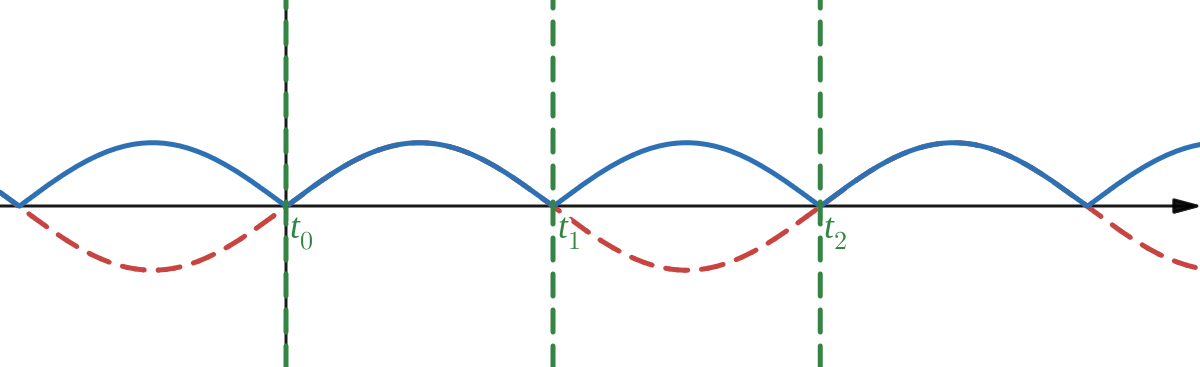
\includegraphics[scale=0.3]{../figures/rect_trans.png}
\end{center}
Abbiamo quindi riempito il secondo semiperiodo come ci eravamo prefissi di fare.

\subsubsection{Circuito rettificatore a doppia semionda con filtro RC}
Concludiamo reintroducendo il condensatore $C$ per "stabilizzare" in qualche modo il voltaggio. Non facciamo il caso con solo $C$, in quanto sarebbe banale ed uguale al caso senza doppia semionda, e passiamo direttamente al filtro RC: \begin{center}
\begin{circuitikz}
	\draw (-3, 1) to[american voltage source, l=$V_s$] (-3, -1)
	-- (-1, -1) to[inductor] (-1, 1) -- (-3, 1);

	\draw (0,2) to[inductor, l=$A$] (0, 0);
	\draw (0,2) to[diode, l=$D_1$] (4,2) -- (4,0);
	\draw (0,0) to[inductor, l=$B$] (0, -2);
	\draw (0,-2) to[diode, l=$D_2$] (4,-2) -- (4,0);
	\draw (0,0) -- (6,0);
	
	\draw(4,2) -- (8,2) to[resistor, l=$R_L$] (8,0) -- (6,0);
	\draw(6,2) to[capacitor, l=$C$] (6,0);
	\node[ground] at(6,0) {};
	\draw (8,2) -- (9, 2);
	\node[anchor=west] at(9,2) {$V_u$};

	\draw (-0.9,0.4) node {$\scriptscriptstyle\bullet$};
	\draw (-0.1,1.4) node {$\scriptscriptstyle\bullet$};
	\draw (-0.1,-0.6) node {$\scriptscriptstyle\bullet$};

	\draw (-0.5,1) -- (-0.5,-1);
\end{circuitikz}
\end{center}

Quello che otteniamo è qundi l'effetto combinato della doppia semionda e del condensatore. Anche in questo caso, quando il diodo entrerà in interdizione, la tensione sul condensatore tendera a scaricarsi sulla resistenza seguendo l'equazione tipica del circuito RC.
Ciò significherà che gli istanti dove $V_s$ salirà sopra il livello raggiunto da $V_u$ e quindi ricaricherà il condensatore (alzando il voltaggio nuovamente fino al valore di picco) accadranno con frequenza doppia (in corrispondenza sia di $t_0$ che di $t_1$, più opportune fasi). 

\newpage

Questo ci permetterà di ridurre al minimo l'effetto del ripple voltage, portando ad una forma d'onda che è molto vicina all'essere costante. 

\begin{center}
	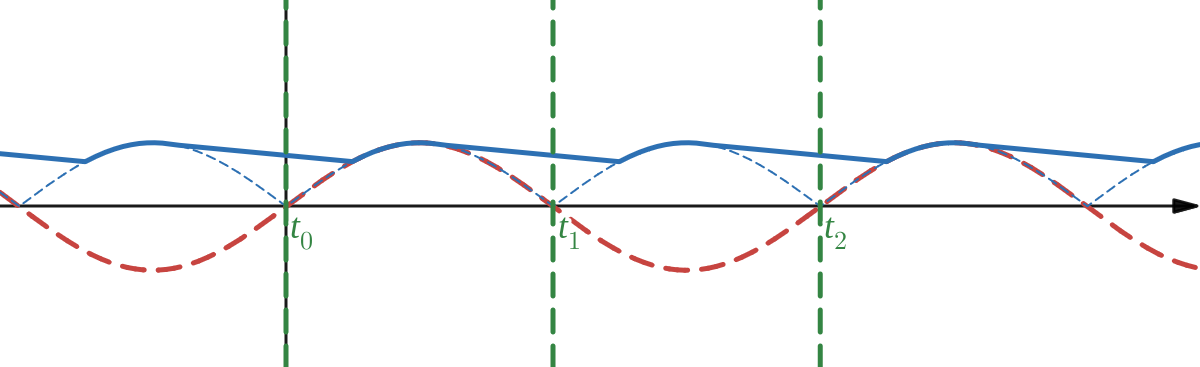
\includegraphics[scale=0.3]{../figures/rect_transcap.png}
\end{center}

\subsubsection{Rettificatore a ponte di Graetz}
Una soluzione alternativa alla doppia semionda col trasformatore (che chiamiamo anche \textit{presa centrale}) è data dall'utilizzo di una particolare configurazione di diodi, detta ponte di \textit{Graetz}.

% ponte di gratez

\subsubsection{Confronto fra tra presa centrale e ponte di Graetz}
Confrontiamo le due soluzioni che abbiamo dato per la rettifica del segnale.

\begin{itemize}
	\item La soluzione a \textbf{presa centrale} per la rettifica della tensione richiede un trasformatore ingombrante e costoso, di cui solo metà avvolgimento per volta è effettivamente in operazione;
	\item La soluzione a \textbf{ponte di Graetz} invece utilizza 4 diodi che lavorano in coppia per risolvere lo stesso problema. Solitamente i diodi sono compatti e leggeri rispetto al trasformatore della presa centrale, per cui si ottiene un circuito più compatto e più leggero.
\end{itemize}

Notiamo quindi in termini numerici quali sono le differenze principali:
\begin{table}[H]
\centering
\begin{tabular}{l|c|c}
\textbf{Caratteristica} & \textbf{Presa Centrale} & \textbf{Ponte di Graetz} \\
\hline
Diodi necessari & 2 & 4 \\
\hline
PIV (Tensione Inversa) & $2V_s$ & $V_s$ \\
\hline
Ingombro/Peso & Elevato (Ferro/Rame) & Ridotto (Efficiente) \\
\hline
Caduta di tensione & $1 \times V_\gamma$ & $2 \times V_\gamma$ \\
\end{tabular}
\end{table}

In conclusione, il ponte di Graetz è lo standard moderno, in quanto il costo di due diodi extra è trascurabile rispetto al risparmio su peso e dimensioni del trasformatore.

Detto questo, il ponte di Graetz non è perfetto: a parte il problema del costo aggiunto dei 4 (2 in più rispetto alla presa centrale) diodi, abbiamo che l’uscita di un ponte di Graetz è unidirezionale, ma fortemente pulsante. Questo significa che si ha comunque un effetto consistente del ripple voltage. Abbiamo che questa fluttuazione di tensione (ondulazione) è inaccettabile per la maggior parte dei circuiti elettronici. Ad esempio:

\begin{itemize}
	\item Nei circuiti \textit{audio}, il ripple voltage comporta un ronzio a $100 \, \mathrm{Hz}$ (in Europa, $120 \, \mathrm{Hz}$ negli Stati Uniti) negli altoparlanti;
	\item Nei circuiti \textit{digitali} si potrebbero avere errori logici: microprocessori che lavorano ad alta frequenza potrebbero riavviarsi se sottoposti a variazione della tensione di alimentazione;
	\item Si potrebbero avere errori di precisione nei circuiti di \textit{misura}, ovvero imprecisioni dei sensori utilizzati.
\end{itemize}

La strategia per risolvere questo problema sarà data in due passaggi:
\begin{enumerate}
	\item \textbf{Filtraggio}: Adottiamo un condensatore per "livellare" le valli di tensione (e questo lo abbiamo già visto, introducendo il filtro RC nei rettificatori studiati);
	\item \textbf{Regolazione}: Introduciamo un diodo \textit{Zener} (visti in 6.1.1) per rendere l’uscita immune alle variazioni del carico. Avevamo già introdotto, infatti, come un diodo di Zener in regime di breakdown può comportarsi come un generatore di tensione costante.
\end{enumerate}

\subsubsection{Rettificatore con diodo Zener}
Vediamo nello specifico come i diodi \textbf{Zener} vengono usati nei rettificatori. Abbiamo che questi sono, di base, componenti con le seguenti caratteristiche:
\begin{itemize}
    \item A differenza dei diodi comuni, il diodo Zener è progettato per lavorare stabilmente nella regione di rottura (\textit{breakdown}) senza danneggiarsi;
	\item In questa zona, la curva $i\text{-}v$ diventa quasi verticale: grandi variazioni di corrente corrispondono a variazioni minime di tensione.
\end{itemize}

Ciò significa che il diodo Zener si comporta come segue:
\begin{itemize}
    \item Si comporta come un normale diodo in polarizzazione diretta.
    \item In polarizzazione inversa, blocca la corrente fino a $V_Z$.
    \item Superata $V_Z$, la tensione ai capi del diodo resta circa costante a $V_Z$.
\end{itemize}

Questo significa che possiamo utilizzare il diodo Zener per effettuare 2 operazioni principali:
\begin{itemize}
    \item \textbf{Riferimento}: il diodo in regime di breakdown fornisce una tensione costante e nota;
    \item \textbf{Protezione}: introducendo un diodo Zener possiamo imitare i picchi di tensione.
\end{itemize}

\newpage

Avremo bisogno di modificare il modello a caduta tensione che avevamo introdotto per il diodo, introducendo la zona di breakdown per voltaggi negativi. 

\begin{center}
	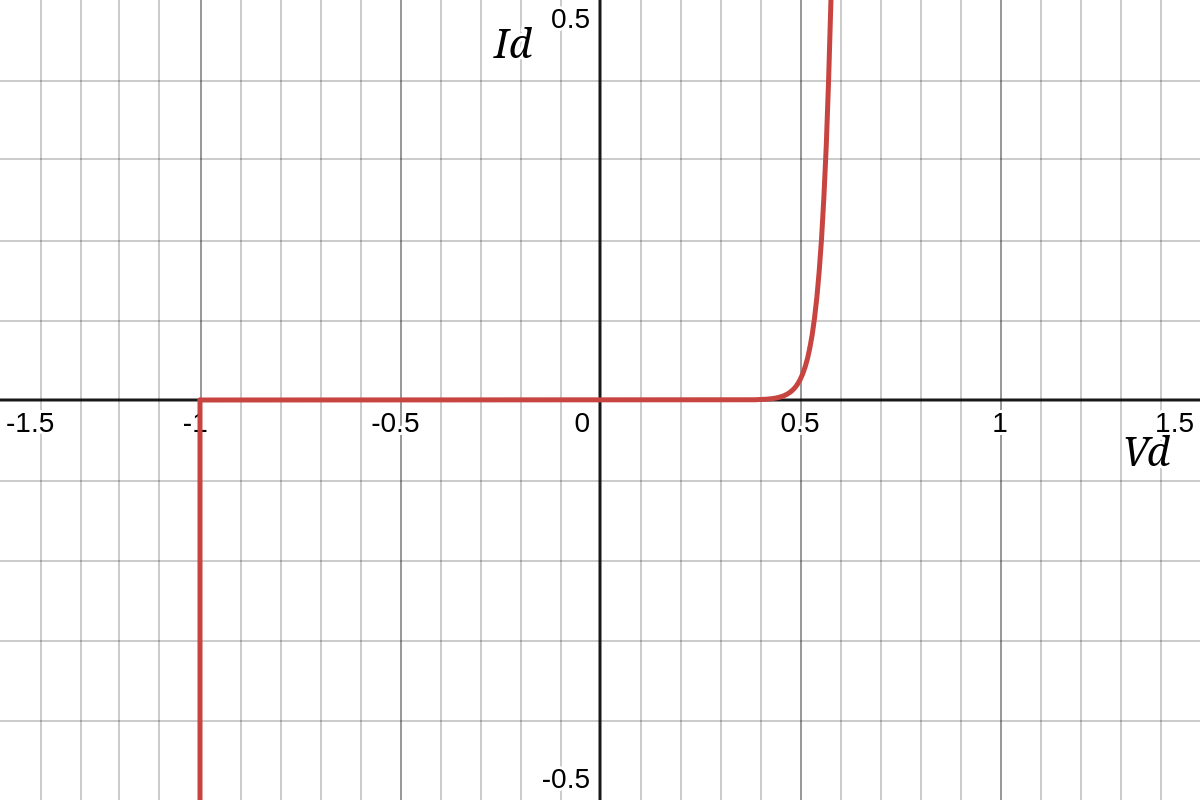
\includegraphics[scale=0.25]{../figures/zener.png}
\end{center}

Il modello a caduta costante cambierà quindi in 3 regioni operative:
\begin{enumerate}
    \item Conduzione in polarizzazione diretta: 
    \[
    V_{AK} = V_\gamma, \quad \text{verificare } I_D \geq 0
    \]

    \item Interdizione:
    \[
    I_D = 0, \quad \text{verificare } -|V_Z| < V_{AK} < V_\gamma
    \]

    \item Conduzione in polarizzazione inversa (breakdown): 
    \[
    V_{AK} = -|V_Z|, \quad \text{verificare } I_D \leq 0
    \]
    Questa è la zona di funzionamento utilizzata per il regolatore.
\end{enumerate} 

\end{document}
